



\section{STUDY 1: CONSRUCT PPG AND GSR DATASET FOR TRAINING EMOTION DETECTION MODEL}
Study 1 focuses on improving a pre-selected dataset consisting of a number of 3-minute videos, spanning a number of emotional states. The aim is to reduce the number of videos in the dataset so that it will contain a smaller number of videos for each emotion which will be the most representative videos of the given emotion.

\subsection{Dataset design}
The dataset used in this study, is a collection of different 3-minute videos spanning a variety of emotional states. Each emotion is represented through a valence and arousal model, which is displayed in \cref{fig:1}. The arousal and valence model is able to represent a total of 28 different emotions, however, a decision has been made to focus on the 14 emotional states, shown in \cref{fig:1}. The model itself is a coordinate system consisting of valence and arousal dimensions. Valence refers to the pleasant–unpleasant quality of a stimulus and ranges from negative to positive, whereas arousal refers to the intensity of a stimulus and ranges from dull to arousing. Using this way of defining emotions, it is possible to map levels of arousal and valence to different emotions. Since there are no actual values on either of the axis in the model, levels of valence and arousal will be used to describe points of the model instead. These levels could for instance be a two-level model, which consists of two levels; low or high. However, this presents a trade-off between accuracy and the difficulty of managing a large number of levels in the dimensions. To this end, a decision has been made, that a 4-level arousal and valence model will be used, where the different levels are defined as very low, low, high and very high, displayed in \cref{fig:2}. By using these levels, it is possible to map to a broader variety of emotions. As a result of this, a total of 16 combinations on the 4-level arousal and valance model needs to be covered. Furthermore, 5 videos for each combination will exist, which is summing up to 80 3-minute videos.

\begin{figure}
\centering
\begin{subfigure}{.5\textwidth}
  \centering
  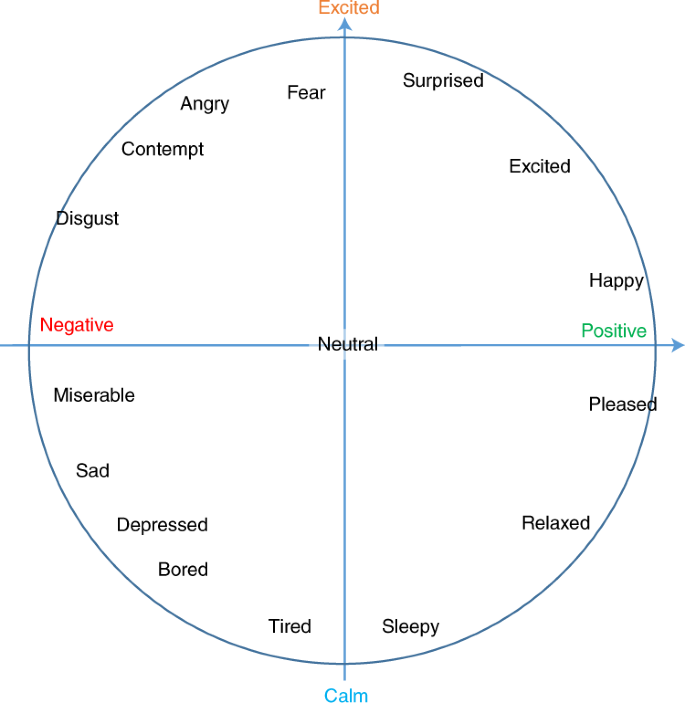
\includegraphics[width=.8\linewidth]{figures/valancearousal.png}
  \caption{Arousal- and valance model}
  \label{fig:1}
\end{subfigure}%
\begin{subfigure}{.5\textwidth}
  \centering
  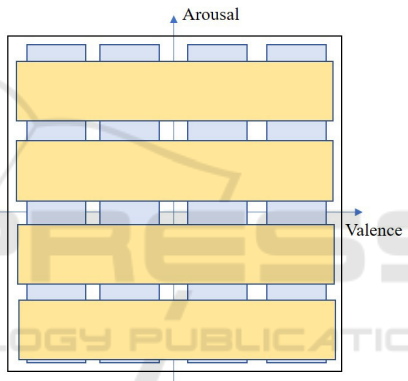
\includegraphics[width=.8\linewidth]{figures/4levelarousal.png}
  \caption{4-level arousal- and valance model}
  \label{fig:2}
\end{subfigure}
\caption{Arousal- and valance model models}
\label{fig:test}
\end{figure}


\subsection{Participants}
xx volunteers from the university community participated in the study. Each participant was showed videos relating one emotion, which means that each session took around 20 minutes to conduct. The participants used in the study, was random people within the computer science department.

\subsection{Procedure}
The study was conducted in a quiet room, while wearing noise-cancellation head-phones, in order to prevent any possible distracting noise. 
Before each session begins, the participants are briefed on the procedure, furthermore they are asked to remain motionless, such that noise in the data is minimized.
Participants watch 5 videos selected for this study, each with a length of 3 minutes. The 5 videos are selected with the intention of capturing a single emotion, which is defined as an emotion category. Participants are asked to pick out the two videos that they feel is the most representative of the given emotion category. Finally participants give an elaboration of why they chose the 2 videos, as the best representatives.
When the sessions are conducted, the 2 videos within each emotion category which where chosen most times are used as part of the custom dataset, while the remaining 3 are discarded.

\subsection{Results}
Conducting this study, the initial 80 video dataset was reduced to 32 videos, consisting of 2 videos for each combination of the 4-level valence and arousal model.